\documentclass[10pt,handout,english]{beamer}
\usetheme{Warsaw}
\usepackage{graphicx}
\usepackage{placeins}
\usepackage{amsmath, amssymb}
\usepackage{tabu}
\usepackage{bbm}
\usepackage{booktabs}
\usepackage[round]{natbib}
\usepackage{bm}
\usepackage{ragged2e}
\usepackage{bbm}
\usepackage{hyperref}
\usepackage{amsmath}
\usepackage{xcolor}
\usepackage[super]{nth}
\hypersetup{
    colorlinks=true,
    linkcolor=blue,
    filecolor=blue,      
    urlcolor=blue,
    citecolor=black,
}

\apptocmd{\frame}{}{\justifying}{} % Allow optional arguments after frame.

\setbeamertemplate{frametitle continuation}{}

\newcommand\setItemnumber[1]{\setcounter{enumi}{\numexpr#1-1\relax}}

\DeclareMathOperator{\tr}{tr}

\newcommand{\ts}{\textsuperscript}
\newcommand{\E}{\mathbb{E}}
\newcommand{\R}{\mathbb{R}}
\newcommand{\F}{\mathcal{F}}
\newcommand{\vertiii}[1]{{\left\vert\kern-0.25ex\left\vert\kern-0.25ex\left\vert #1 
    \right\vert\kern-0.25ex\right\vert\kern-0.25ex\right\vert}}


\title[]{Sparse linear models in high dimensions}
\author[Kaveh S. Nobari]{Kaveh S. Nobari}
\institute[]{Lectures in High-Dimensional Statistics}
\date[27/10/2020]
{Department of Mathematics and Statistics\\ Lancaster University}
	

\begin{document}
\begin{frame}
\titlepage
\end{frame}


\begin{frame}{Contents}
\tableofcontents
\end{frame}

\begin{frame}[allowframebreaks]{Motivation}
\begin{block}{Classical vs High-Dimensional asymptotics}
\begin{itemize}
 \item \textcolor{red}{Classical:} low-dimensional settings, in which the number of predictors  $d$ is substantially less than the sample size $n$ - i.e., $d\ll n$.
\item\textcolor{red}{High-dimensional:} High-dimensional regime allows for scaling such that $d\asymp n$ or even $d\gg n$.
\end{itemize}
\end{block}

In the case that $d\gg n$, if the model lacks any additional structure, then there is no hope of obtaining consistent estimators when the ratio $d/n$ stays bounded away from zero. Therefore, when working in settings in which $d>n$, it is necessary to impose additional structure on the unknown regression vector $\theta^*\in \R^d$.
\end{frame}


\section{Problem formulation and applications}
\frame{\tableofcontents[currentsection]}
\begin{frame}[allowframebreaks]
Let $\theta^*\in \R^d$ be an unknown vector, and suppose we observe a vector $y\in\R^n$ and a matrix $X\in \R^{n\times d}$, such that $X=[x_1',\cdots,x_n']'$ that are linked via the linear model
\[
y=X\theta^*+\varepsilon
\]
where $\varepsilon \in \R^{n}$ is the noise vector. This model can be written in any of the following scalar forms
\begin{align*}
y_i=\langle x_i,\theta^*\rangle+\varepsilon_i,\quad i=1,\cdots,n,\\
y_i=x_i'\theta+\varepsilon_i,\quad i=1,\cdots,n,\\
\end{align*}
where $\langle x_i,\theta^*\rangle=\sum\limits_{i=1}^{n}x_{ij}\theta_j^*$ denotes the Euclidean inner product.

The focus of this presentation is to consider the cases where $n<d$. We first consider the \textcolor{red}{noiseless linear model}, such that $\epsilon=0$, in which we may model the response variable as
\[
y=X\theta^{*}
\]
which when $n<d$ defines an undetermined linear system, and the goal is to understand the \textcolor{red}{structure of its sparse solutions}.
\end{frame}


\subsection{Different sparsity models}
\frame{\tableofcontents[currentsection, currentsubsection]}
%------------------------------------------------
\begin{frame}[allowframebreaks]
When $d>n$, it is impossible to obtain any meaningful estimate of $\theta^*$ unless the model is equipped with some form of low-dimensional structure. First, we consider the simplest case, namely the \textcolor{red}{hard sparsity} assumption:

\begin{block}{Hard sparsity assumption}
The simplest kind of structure is the hard sparsity assumption that the set
\[
S(\theta^*):=\{j\in\{1,\cdots,d\}\mid\theta_j^*\neq 0\}.
\]
which is known as the support of $\theta^*$ and has cardinality $s:=\lvert S(\theta^*)\rvert$, where $s\ll d$.¸
\end{block}
The problem with the hard sparsity assumption is that it is \textcolor{red}{overly restrictive}, which motivates considering the \textcolor{red}{weak sparsity} assumption.
\begin{definition}
A vector $\theta^*$ is weakly sparse if it can be closely approximated by a sparse vector.
\end{definition}
One way to formalize such an idea is via the $l_q$-norms. For a parameter $q\in[0,1]$ and radius $R_1>0$, consider the $l_q$-ball set
\[
B_q(R_q)=\left\{\theta\in\R^d\mid\sum\limits_{j=1}^{d}\lvert \theta_j\rvert^q\leq R_q\right\}
\]  
is one with radius $R_q$. As it is evident from the below figures for $q\in[0,1)$, it is not a ball in the strict sense, since it a non-convex set. When $q=0$, this is the case of the \textquotedblleft improper\textquotedblright{ }$l_0$-norm, and any vector $\theta^*\in B_0(R_0)$ can have at most $s=R_0$ non-zero entries. For values of $q\in (0,1]$, membership in the set $B_q(R_q)$ has different interpretations, one of which involves, how quickly the ordered coefficients
\[
\lvert \theta_{(1)}^*\rvert\geq\lvert \theta_{(2)}^*\rvert\geq\cdots\geq\lvert \theta_{(d)}^*\rvert
\]
decay.
\end{frame}
\begin{frame}
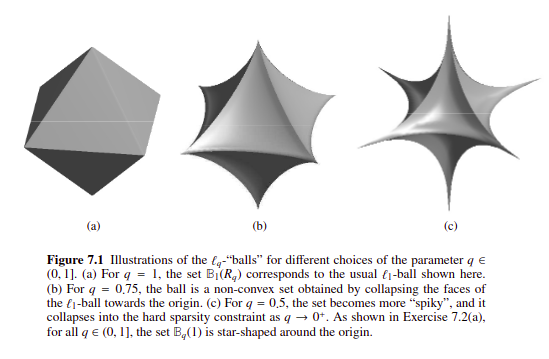
\includegraphics[width=\textwidth, height=\textheight]{lqballs.png}
\end{frame}
\subsection{Applications of sparse linear models}
\frame{\tableofcontents[currentsection, currentsubsection]}

\begin{frame}[allowframebreaks]
\textbf{Example (Gaussian sequence models):}
Suppose we observed $\{y_1,\cdots,y_n\}$ where
\[
y_i=\theta_i^*+\epsilon\varepsilon_i,
\]
where $\varepsilon_i\sim N(0,1)$ and $\epsilon=\frac{\sigma}{\sqrt{n}}$, where the variance is divided by $n$, as it corresponds to taking $n$ i.i.d variables and taking their average. In this case, it is evident that $n=d$ and as $n\to\infty$, so does $d\to\infty$. It is clearly evident that in the general linear model introduced earlier - i.e.
\[
y=X\theta^*+\varepsilon
\]
$X=I_n$.

\textbf{Example (Signal denoising in orthonormal bases):} Sparsity plays an important role in signal processing, both for compression and for denoising of signals. Suppose we have the noisy observations $\tilde{y}=(\tilde{y}_1,\cdots,\tilde{y}_n)'$.
\[
\tilde{y}=\beta^*+\tilde{\varepsilon}
\]
where the vector $\beta^*\in\R^d$ represents the signal, while $\tilde{\varepsilon}$ is some kind of additive noise. Denoising $\tilde{y}$ implies that constructing $\beta^*$ as accurately as possible, which mean producing a representation of $\beta^*$ that can be stored compactly than its original representation.

Many classes of signals exhibit sparsity when transformed into the appropriate basis, such as a wavelet basis. Such transform can be represented as an orthonormal matrix $\Psi\in\R^{d\times d}$, constructed so that 
\[
\theta^*:=\Psi'\beta^*\in \R^d
\]
corresponds to the vector of transformed coefficients. If $\theta^*$ is known to be sparse then only a fraction of the coefficients, say the $s<d$ largest coefficients in absolute value can be retained.

In the transformed space, the model takes the form
\[
y =\theta^*+\varepsilon
\]
where $y=\Psi'\tilde{y}$, and $\Psi'\tilde{\varepsilon}$. If $\tilde{\varepsilon}\sim N(0,\sigma^2)$, then it is invariant under orthogonal transformation and the original and transformed observations $\tilde{y}$ and $y$ are examples of Gaussian sequence models touched in the earlier example, both with $n=d$. If $\theta^*$ is known to be sparse then it is natural to consider estimators based on thresholding. \citet{wainwright2019high} shows that for a hard threshold of $\lambda>0$, we may have \textcolor{red}{hard-threshold} or \textcolor{red}{soft-threshold} estimates of $\theta^*$.


\textbf{Example (Lifting and non-linear functions):} Consider the $n$ pair of observations $\{(y_i,t_i)\}_{i=1}^n$, where each pair is lined via the model 
\[
y_i=f(t_i;\theta)+\varepsilon_i,
\]
where 
\[
f(t_i;\theta)=\theta_1+\theta_2t_i+\theta_3t_i^2+\cdots+\theta_{k+1}t_i^k.
\]
This non-linear problem can be converted into an instance of linear regression model, by defining the $n\times(k+1)$ matrix
\[
X=
\begin{bmatrix}
1&t_1&t_1^2&\cdots&t_1^k\\
1&t_2&t_2^2&\cdots&t_2^k\\
\vdots&\vdots&\vdots&\ddots&\vdots\\
1&t_n&t_n^2&\cdots&t_n^k
\end{bmatrix}
\]
which once again leads to the general linear model
\[
y=X\theta+\varepsilon.
\]
If we were to extend the univariate function above to a multivariate functions in  $D$ dimensions, there are $\binom{k}{D}$ possible multinomials of degree $k$ in dimension $D$. This leads to an exponentially growing model with dimension of the magnitude $D^k$, so that the sparsity assumptions become essential.
\end{frame}

\section{Recovery in noiseless setting}
\frame{\tableofcontents[currentsection]}

\begin{frame}[allowframebreaks]
To build intuition, we start we the simplest case were there observations are noiseless. Essentially, we wish to find a solution $\theta$ to the linear system
\[
y=X\theta,
\]
where $y\in\R^n$ and $X\in\R^{n\times d}$, such that $d>n$. When $d>n$, this is an \textcolor{red}{undetermined} set of linear equations, so there is a whole subspace of solutions. 

If we have a \textcolor{red}{sparse solution} that means that there is a vector $\theta^*\in\R^d$, with at most $s\ll d$ non-zero entries and such that $y=X\theta^*$.

The goal is to find this sparse solution to the linear system.
\end{frame}

\subsection{$l_1$-based relaxation}
\frame{\tableofcontents[currentsection,currentsubsection]}

\begin{frame}[allowframebreaks]
This problem can be expressed as  a non-convex optimization problem involving the $l_0$-\textquotedblleft norm\textquotedblright. 

\textbf{Question:} The $l_0$-norm has been put in quotation marks, as it is not considered a \underline{proper} norm. Why is that?

Let us define
\[
\lVert \theta\rVert_0:=\sum\limits_{j=1}^{d}\mathbbm{1}[\theta_j\neq 0]
\] 
where $\mathbbm{1}$ is an indicator function. Thus, the optimization problem is
\[
\min_{\theta\in\R^d}\lVert \theta\rVert_0\quad\text{such that}\quad X\theta=y
\]
Solving this leads to obtaining a solution to the linear equations that has the fewest number of non-zero entries. How can we solve the above optimization problem? The constraint set is simply a subspace, but the cost function is \textcolor{red}{non-differentiable} and \textcolor{red}{non-convex}.
\end{frame}
\begin{frame}[allowframebreaks]
\begin{block}{Algorithm for solving the $l_0$ optimization problem}
\begin{enumerate}
\item[1)]  For each subset $S\subset \{1,\cdots,d\}$, we form the matrix $X_{S}\in\R^{\lvert S\rvert}$, consisting of the columns of $X$ indexed by S.
\item[2)] Examine the linear system $y=X_S\theta$ to see whether it has a solution $\theta\in\R^{\lvert S\rvert}$.
\item[3)] Iterate over subsets in increasing cardinality, then the first solution found would be the sparsest solution.
\end{enumerate}
\end{block}

What would be the computational cost of this optimisation approach be? If the sparsest solution contained $s$ non-zero entries, then we would have to search over at least 
\[
\sum\limits_{j=1}^{s-1}\binom{d}{j}
\]
subsets before finding it.

The next solution is to replace $l_0$ with the \textcolor{red}{nearest convex member} of the $l_q$ family, namely the $l_1$ norm. 
\begin{definition}[Convex relaxation]
When a non-convex optimization problem is approximated by a convex programme.
\end{definition}
In this setting this leads to the optimization problem
\[
\min_{\theta\in\R^d}\lVert \theta\rVert_1\quad\text{such that}\quad X\theta=y.
\]
The constraint sex is a subspace (hence convex), and the cost function is piecewise linear and thus convex as well. The $l_1$ optimisation problem is a linear programme, since any piecewise linear convex cost can always be reformulated as the maximum of a collection of linear functions. The above optimisation problem is referred to as \textcolor{red}{basis pursuit linear programme}.
\end{frame}


\subsection{Exact recovery and restricted null space}
\frame{\tableofcontents[currentsection,currentsubsection]}

\begin{frame}[allowframebreaks]
When is solving the basis pursuit problem
\[
\min_{\theta\in\R^d}\lVert \theta\rVert_1\quad\text{such that}\quad X\theta=y.
\]
equivalent to solving the $l_0$ problem below?
\[
\min_{\theta\in\R^d}\lVert \theta\rVert_0\quad\text{such that}\quad X\theta=y
\]
Suppose $\theta^*=\R^d$ such that $y=X\theta^*$. Moreover, the vector $\theta^*$ has the support $S\subset\{1,2,\cdots,d\}$, which means that $\theta^*_j=0$ for all $j\in S^C$.

The success of the basis pursuit should depend on how the nullspace of $X$ is related to this support, where by definition
\[
\text{null}(X):=\{\Delta\in\R^d\mid X\Delta=0\}.
\]
Since $X\theta^*=y$ by assumption, any vector of the form $\theta^*+\Delta$ for some $\Delta\in\text{null}(X)$ is feasible for the basis pursuit programme.
\end{frame}
\subsection{Sufficient conditions for restricted null space}
\frame{\tableofcontents[currentsection,currentsubsection]}


\section{Estimation in noisy settings}
\subsection{Restricted eigenvalue condition}
\frame{\tableofcontents[currentsection,currentsubsection]}

\subsection{Bounds on $l_2$-error for hard sparse models}
\frame{\tableofcontents[currentsubsection]}

\subsection{Restricted nullspace and eigenvalues for random designs}
\frame{\tableofcontents[currentsubsection]}

\section{Bounds on prediction error}
\frame{\tableofcontents[currentsection]}

\section{Variable or subset selection}
\subsection{Variable selection consistency for the Lasso}
\frame{\tableofcontents[currentsection]}

\subsection{Proof of Theorem 7.21}
\frame{\tableofcontents[currentsection]}


\begin{frame}[allowframebreaks]
\frametitle{References}
\bibliographystyle{apa}
\bibliography{References_HDStat}
\end{frame}

\end{document}